
% Default to the notebook output style

    


% Inherit from the specified cell style.




    
\documentclass[11pt]{article}

    
    
    \usepackage[T1]{fontenc}
    % Nicer default font (+ math font) than Computer Modern for most use cases
    \usepackage{mathpazo}

    % Basic figure setup, for now with no caption control since it's done
    % automatically by Pandoc (which extracts ![](path) syntax from Markdown).
    \usepackage{graphicx}
    % We will generate all images so they have a width \maxwidth. This means
    % that they will get their normal width if they fit onto the page, but
    % are scaled down if they would overflow the margins.
    \makeatletter
    \def\maxwidth{\ifdim\Gin@nat@width>\linewidth\linewidth
    \else\Gin@nat@width\fi}
    \makeatother
    \let\Oldincludegraphics\includegraphics
    % Set max figure width to be 80% of text width, for now hardcoded.
    \renewcommand{\includegraphics}[1]{\Oldincludegraphics[width=.8\maxwidth]{#1}}
    % Ensure that by default, figures have no caption (until we provide a
    % proper Figure object with a Caption API and a way to capture that
    % in the conversion process - todo).
    \usepackage{caption}
    \DeclareCaptionLabelFormat{nolabel}{}
    \captionsetup{labelformat=nolabel}

    \usepackage{adjustbox} % Used to constrain images to a maximum size 
    \usepackage{xcolor} % Allow colors to be defined
    \usepackage{enumerate} % Needed for markdown enumerations to work
    \usepackage{geometry} % Used to adjust the document margins
    \usepackage{amsmath} % Equations
    \usepackage{amssymb} % Equations
    \usepackage{textcomp} % defines textquotesingle
    % Hack from http://tex.stackexchange.com/a/47451/13684:
    \AtBeginDocument{%
        \def\PYZsq{\textquotesingle}% Upright quotes in Pygmentized code
    }
    \usepackage{upquote} % Upright quotes for verbatim code
    \usepackage{eurosym} % defines \euro
    \usepackage[mathletters]{ucs} % Extended unicode (utf-8) support
    \usepackage[utf8x]{inputenc} % Allow utf-8 characters in the tex document
    \usepackage{fancyvrb} % verbatim replacement that allows latex
    \usepackage{grffile} % extends the file name processing of package graphics 
                         % to support a larger range 
    % The hyperref package gives us a pdf with properly built
    % internal navigation ('pdf bookmarks' for the table of contents,
    % internal cross-reference links, web links for URLs, etc.)
    \usepackage{hyperref}
    \usepackage{longtable} % longtable support required by pandoc >1.10
    \usepackage{booktabs}  % table support for pandoc > 1.12.2
    \usepackage[inline]{enumitem} % IRkernel/repr support (it uses the enumerate* environment)
    \usepackage[normalem]{ulem} % ulem is needed to support strikethroughs (\sout)
                                % normalem makes italics be italics, not underlines
    

    
    
    % Colors for the hyperref package
    \definecolor{urlcolor}{rgb}{0,.145,.698}
    \definecolor{linkcolor}{rgb}{.71,0.21,0.01}
    \definecolor{citecolor}{rgb}{.12,.54,.11}

    % ANSI colors
    \definecolor{ansi-black}{HTML}{3E424D}
    \definecolor{ansi-black-intense}{HTML}{282C36}
    \definecolor{ansi-red}{HTML}{E75C58}
    \definecolor{ansi-red-intense}{HTML}{B22B31}
    \definecolor{ansi-green}{HTML}{00A250}
    \definecolor{ansi-green-intense}{HTML}{007427}
    \definecolor{ansi-yellow}{HTML}{DDB62B}
    \definecolor{ansi-yellow-intense}{HTML}{B27D12}
    \definecolor{ansi-blue}{HTML}{208FFB}
    \definecolor{ansi-blue-intense}{HTML}{0065CA}
    \definecolor{ansi-magenta}{HTML}{D160C4}
    \definecolor{ansi-magenta-intense}{HTML}{A03196}
    \definecolor{ansi-cyan}{HTML}{60C6C8}
    \definecolor{ansi-cyan-intense}{HTML}{258F8F}
    \definecolor{ansi-white}{HTML}{C5C1B4}
    \definecolor{ansi-white-intense}{HTML}{A1A6B2}

    % commands and environments needed by pandoc snippets
    % extracted from the output of `pandoc -s`
    \providecommand{\tightlist}{%
      \setlength{\itemsep}{0pt}\setlength{\parskip}{0pt}}
    \DefineVerbatimEnvironment{Highlighting}{Verbatim}{commandchars=\\\{\}}
    % Add ',fontsize=\small' for more characters per line
    \newenvironment{Shaded}{}{}
    \newcommand{\KeywordTok}[1]{\textcolor[rgb]{0.00,0.44,0.13}{\textbf{{#1}}}}
    \newcommand{\DataTypeTok}[1]{\textcolor[rgb]{0.56,0.13,0.00}{{#1}}}
    \newcommand{\DecValTok}[1]{\textcolor[rgb]{0.25,0.63,0.44}{{#1}}}
    \newcommand{\BaseNTok}[1]{\textcolor[rgb]{0.25,0.63,0.44}{{#1}}}
    \newcommand{\FloatTok}[1]{\textcolor[rgb]{0.25,0.63,0.44}{{#1}}}
    \newcommand{\CharTok}[1]{\textcolor[rgb]{0.25,0.44,0.63}{{#1}}}
    \newcommand{\StringTok}[1]{\textcolor[rgb]{0.25,0.44,0.63}{{#1}}}
    \newcommand{\CommentTok}[1]{\textcolor[rgb]{0.38,0.63,0.69}{\textit{{#1}}}}
    \newcommand{\OtherTok}[1]{\textcolor[rgb]{0.00,0.44,0.13}{{#1}}}
    \newcommand{\AlertTok}[1]{\textcolor[rgb]{1.00,0.00,0.00}{\textbf{{#1}}}}
    \newcommand{\FunctionTok}[1]{\textcolor[rgb]{0.02,0.16,0.49}{{#1}}}
    \newcommand{\RegionMarkerTok}[1]{{#1}}
    \newcommand{\ErrorTok}[1]{\textcolor[rgb]{1.00,0.00,0.00}{\textbf{{#1}}}}
    \newcommand{\NormalTok}[1]{{#1}}
    
    % Additional commands for more recent versions of Pandoc
    \newcommand{\ConstantTok}[1]{\textcolor[rgb]{0.53,0.00,0.00}{{#1}}}
    \newcommand{\SpecialCharTok}[1]{\textcolor[rgb]{0.25,0.44,0.63}{{#1}}}
    \newcommand{\VerbatimStringTok}[1]{\textcolor[rgb]{0.25,0.44,0.63}{{#1}}}
    \newcommand{\SpecialStringTok}[1]{\textcolor[rgb]{0.73,0.40,0.53}{{#1}}}
    \newcommand{\ImportTok}[1]{{#1}}
    \newcommand{\DocumentationTok}[1]{\textcolor[rgb]{0.73,0.13,0.13}{\textit{{#1}}}}
    \newcommand{\AnnotationTok}[1]{\textcolor[rgb]{0.38,0.63,0.69}{\textbf{\textit{{#1}}}}}
    \newcommand{\CommentVarTok}[1]{\textcolor[rgb]{0.38,0.63,0.69}{\textbf{\textit{{#1}}}}}
    \newcommand{\VariableTok}[1]{\textcolor[rgb]{0.10,0.09,0.49}{{#1}}}
    \newcommand{\ControlFlowTok}[1]{\textcolor[rgb]{0.00,0.44,0.13}{\textbf{{#1}}}}
    \newcommand{\OperatorTok}[1]{\textcolor[rgb]{0.40,0.40,0.40}{{#1}}}
    \newcommand{\BuiltInTok}[1]{{#1}}
    \newcommand{\ExtensionTok}[1]{{#1}}
    \newcommand{\PreprocessorTok}[1]{\textcolor[rgb]{0.74,0.48,0.00}{{#1}}}
    \newcommand{\AttributeTok}[1]{\textcolor[rgb]{0.49,0.56,0.16}{{#1}}}
    \newcommand{\InformationTok}[1]{\textcolor[rgb]{0.38,0.63,0.69}{\textbf{\textit{{#1}}}}}
    \newcommand{\WarningTok}[1]{\textcolor[rgb]{0.38,0.63,0.69}{\textbf{\textit{{#1}}}}}
    
    
    % Define a nice break command that doesn't care if a line doesn't already
    % exist.
    \def\br{\hspace*{\fill} \\* }
    % Math Jax compatability definitions
    \def\gt{>}
    \def\lt{<}
    % Document parameters
    \title{OpenCV-Python Tutorials}
    
    
    

    % Pygments definitions
    
\makeatletter
\def\PY@reset{\let\PY@it=\relax \let\PY@bf=\relax%
    \let\PY@ul=\relax \let\PY@tc=\relax%
    \let\PY@bc=\relax \let\PY@ff=\relax}
\def\PY@tok#1{\csname PY@tok@#1\endcsname}
\def\PY@toks#1+{\ifx\relax#1\empty\else%
    \PY@tok{#1}\expandafter\PY@toks\fi}
\def\PY@do#1{\PY@bc{\PY@tc{\PY@ul{%
    \PY@it{\PY@bf{\PY@ff{#1}}}}}}}
\def\PY#1#2{\PY@reset\PY@toks#1+\relax+\PY@do{#2}}

\expandafter\def\csname PY@tok@w\endcsname{\def\PY@tc##1{\textcolor[rgb]{0.73,0.73,0.73}{##1}}}
\expandafter\def\csname PY@tok@c\endcsname{\let\PY@it=\textit\def\PY@tc##1{\textcolor[rgb]{0.25,0.50,0.50}{##1}}}
\expandafter\def\csname PY@tok@cp\endcsname{\def\PY@tc##1{\textcolor[rgb]{0.74,0.48,0.00}{##1}}}
\expandafter\def\csname PY@tok@k\endcsname{\let\PY@bf=\textbf\def\PY@tc##1{\textcolor[rgb]{0.00,0.50,0.00}{##1}}}
\expandafter\def\csname PY@tok@kp\endcsname{\def\PY@tc##1{\textcolor[rgb]{0.00,0.50,0.00}{##1}}}
\expandafter\def\csname PY@tok@kt\endcsname{\def\PY@tc##1{\textcolor[rgb]{0.69,0.00,0.25}{##1}}}
\expandafter\def\csname PY@tok@o\endcsname{\def\PY@tc##1{\textcolor[rgb]{0.40,0.40,0.40}{##1}}}
\expandafter\def\csname PY@tok@ow\endcsname{\let\PY@bf=\textbf\def\PY@tc##1{\textcolor[rgb]{0.67,0.13,1.00}{##1}}}
\expandafter\def\csname PY@tok@nb\endcsname{\def\PY@tc##1{\textcolor[rgb]{0.00,0.50,0.00}{##1}}}
\expandafter\def\csname PY@tok@nf\endcsname{\def\PY@tc##1{\textcolor[rgb]{0.00,0.00,1.00}{##1}}}
\expandafter\def\csname PY@tok@nc\endcsname{\let\PY@bf=\textbf\def\PY@tc##1{\textcolor[rgb]{0.00,0.00,1.00}{##1}}}
\expandafter\def\csname PY@tok@nn\endcsname{\let\PY@bf=\textbf\def\PY@tc##1{\textcolor[rgb]{0.00,0.00,1.00}{##1}}}
\expandafter\def\csname PY@tok@ne\endcsname{\let\PY@bf=\textbf\def\PY@tc##1{\textcolor[rgb]{0.82,0.25,0.23}{##1}}}
\expandafter\def\csname PY@tok@nv\endcsname{\def\PY@tc##1{\textcolor[rgb]{0.10,0.09,0.49}{##1}}}
\expandafter\def\csname PY@tok@no\endcsname{\def\PY@tc##1{\textcolor[rgb]{0.53,0.00,0.00}{##1}}}
\expandafter\def\csname PY@tok@nl\endcsname{\def\PY@tc##1{\textcolor[rgb]{0.63,0.63,0.00}{##1}}}
\expandafter\def\csname PY@tok@ni\endcsname{\let\PY@bf=\textbf\def\PY@tc##1{\textcolor[rgb]{0.60,0.60,0.60}{##1}}}
\expandafter\def\csname PY@tok@na\endcsname{\def\PY@tc##1{\textcolor[rgb]{0.49,0.56,0.16}{##1}}}
\expandafter\def\csname PY@tok@nt\endcsname{\let\PY@bf=\textbf\def\PY@tc##1{\textcolor[rgb]{0.00,0.50,0.00}{##1}}}
\expandafter\def\csname PY@tok@nd\endcsname{\def\PY@tc##1{\textcolor[rgb]{0.67,0.13,1.00}{##1}}}
\expandafter\def\csname PY@tok@s\endcsname{\def\PY@tc##1{\textcolor[rgb]{0.73,0.13,0.13}{##1}}}
\expandafter\def\csname PY@tok@sd\endcsname{\let\PY@it=\textit\def\PY@tc##1{\textcolor[rgb]{0.73,0.13,0.13}{##1}}}
\expandafter\def\csname PY@tok@si\endcsname{\let\PY@bf=\textbf\def\PY@tc##1{\textcolor[rgb]{0.73,0.40,0.53}{##1}}}
\expandafter\def\csname PY@tok@se\endcsname{\let\PY@bf=\textbf\def\PY@tc##1{\textcolor[rgb]{0.73,0.40,0.13}{##1}}}
\expandafter\def\csname PY@tok@sr\endcsname{\def\PY@tc##1{\textcolor[rgb]{0.73,0.40,0.53}{##1}}}
\expandafter\def\csname PY@tok@ss\endcsname{\def\PY@tc##1{\textcolor[rgb]{0.10,0.09,0.49}{##1}}}
\expandafter\def\csname PY@tok@sx\endcsname{\def\PY@tc##1{\textcolor[rgb]{0.00,0.50,0.00}{##1}}}
\expandafter\def\csname PY@tok@m\endcsname{\def\PY@tc##1{\textcolor[rgb]{0.40,0.40,0.40}{##1}}}
\expandafter\def\csname PY@tok@gh\endcsname{\let\PY@bf=\textbf\def\PY@tc##1{\textcolor[rgb]{0.00,0.00,0.50}{##1}}}
\expandafter\def\csname PY@tok@gu\endcsname{\let\PY@bf=\textbf\def\PY@tc##1{\textcolor[rgb]{0.50,0.00,0.50}{##1}}}
\expandafter\def\csname PY@tok@gd\endcsname{\def\PY@tc##1{\textcolor[rgb]{0.63,0.00,0.00}{##1}}}
\expandafter\def\csname PY@tok@gi\endcsname{\def\PY@tc##1{\textcolor[rgb]{0.00,0.63,0.00}{##1}}}
\expandafter\def\csname PY@tok@gr\endcsname{\def\PY@tc##1{\textcolor[rgb]{1.00,0.00,0.00}{##1}}}
\expandafter\def\csname PY@tok@ge\endcsname{\let\PY@it=\textit}
\expandafter\def\csname PY@tok@gs\endcsname{\let\PY@bf=\textbf}
\expandafter\def\csname PY@tok@gp\endcsname{\let\PY@bf=\textbf\def\PY@tc##1{\textcolor[rgb]{0.00,0.00,0.50}{##1}}}
\expandafter\def\csname PY@tok@go\endcsname{\def\PY@tc##1{\textcolor[rgb]{0.53,0.53,0.53}{##1}}}
\expandafter\def\csname PY@tok@gt\endcsname{\def\PY@tc##1{\textcolor[rgb]{0.00,0.27,0.87}{##1}}}
\expandafter\def\csname PY@tok@err\endcsname{\def\PY@bc##1{\setlength{\fboxsep}{0pt}\fcolorbox[rgb]{1.00,0.00,0.00}{1,1,1}{\strut ##1}}}
\expandafter\def\csname PY@tok@kc\endcsname{\let\PY@bf=\textbf\def\PY@tc##1{\textcolor[rgb]{0.00,0.50,0.00}{##1}}}
\expandafter\def\csname PY@tok@kd\endcsname{\let\PY@bf=\textbf\def\PY@tc##1{\textcolor[rgb]{0.00,0.50,0.00}{##1}}}
\expandafter\def\csname PY@tok@kn\endcsname{\let\PY@bf=\textbf\def\PY@tc##1{\textcolor[rgb]{0.00,0.50,0.00}{##1}}}
\expandafter\def\csname PY@tok@kr\endcsname{\let\PY@bf=\textbf\def\PY@tc##1{\textcolor[rgb]{0.00,0.50,0.00}{##1}}}
\expandafter\def\csname PY@tok@bp\endcsname{\def\PY@tc##1{\textcolor[rgb]{0.00,0.50,0.00}{##1}}}
\expandafter\def\csname PY@tok@fm\endcsname{\def\PY@tc##1{\textcolor[rgb]{0.00,0.00,1.00}{##1}}}
\expandafter\def\csname PY@tok@vc\endcsname{\def\PY@tc##1{\textcolor[rgb]{0.10,0.09,0.49}{##1}}}
\expandafter\def\csname PY@tok@vg\endcsname{\def\PY@tc##1{\textcolor[rgb]{0.10,0.09,0.49}{##1}}}
\expandafter\def\csname PY@tok@vi\endcsname{\def\PY@tc##1{\textcolor[rgb]{0.10,0.09,0.49}{##1}}}
\expandafter\def\csname PY@tok@vm\endcsname{\def\PY@tc##1{\textcolor[rgb]{0.10,0.09,0.49}{##1}}}
\expandafter\def\csname PY@tok@sa\endcsname{\def\PY@tc##1{\textcolor[rgb]{0.73,0.13,0.13}{##1}}}
\expandafter\def\csname PY@tok@sb\endcsname{\def\PY@tc##1{\textcolor[rgb]{0.73,0.13,0.13}{##1}}}
\expandafter\def\csname PY@tok@sc\endcsname{\def\PY@tc##1{\textcolor[rgb]{0.73,0.13,0.13}{##1}}}
\expandafter\def\csname PY@tok@dl\endcsname{\def\PY@tc##1{\textcolor[rgb]{0.73,0.13,0.13}{##1}}}
\expandafter\def\csname PY@tok@s2\endcsname{\def\PY@tc##1{\textcolor[rgb]{0.73,0.13,0.13}{##1}}}
\expandafter\def\csname PY@tok@sh\endcsname{\def\PY@tc##1{\textcolor[rgb]{0.73,0.13,0.13}{##1}}}
\expandafter\def\csname PY@tok@s1\endcsname{\def\PY@tc##1{\textcolor[rgb]{0.73,0.13,0.13}{##1}}}
\expandafter\def\csname PY@tok@mb\endcsname{\def\PY@tc##1{\textcolor[rgb]{0.40,0.40,0.40}{##1}}}
\expandafter\def\csname PY@tok@mf\endcsname{\def\PY@tc##1{\textcolor[rgb]{0.40,0.40,0.40}{##1}}}
\expandafter\def\csname PY@tok@mh\endcsname{\def\PY@tc##1{\textcolor[rgb]{0.40,0.40,0.40}{##1}}}
\expandafter\def\csname PY@tok@mi\endcsname{\def\PY@tc##1{\textcolor[rgb]{0.40,0.40,0.40}{##1}}}
\expandafter\def\csname PY@tok@il\endcsname{\def\PY@tc##1{\textcolor[rgb]{0.40,0.40,0.40}{##1}}}
\expandafter\def\csname PY@tok@mo\endcsname{\def\PY@tc##1{\textcolor[rgb]{0.40,0.40,0.40}{##1}}}
\expandafter\def\csname PY@tok@ch\endcsname{\let\PY@it=\textit\def\PY@tc##1{\textcolor[rgb]{0.25,0.50,0.50}{##1}}}
\expandafter\def\csname PY@tok@cm\endcsname{\let\PY@it=\textit\def\PY@tc##1{\textcolor[rgb]{0.25,0.50,0.50}{##1}}}
\expandafter\def\csname PY@tok@cpf\endcsname{\let\PY@it=\textit\def\PY@tc##1{\textcolor[rgb]{0.25,0.50,0.50}{##1}}}
\expandafter\def\csname PY@tok@c1\endcsname{\let\PY@it=\textit\def\PY@tc##1{\textcolor[rgb]{0.25,0.50,0.50}{##1}}}
\expandafter\def\csname PY@tok@cs\endcsname{\let\PY@it=\textit\def\PY@tc##1{\textcolor[rgb]{0.25,0.50,0.50}{##1}}}

\def\PYZbs{\char`\\}
\def\PYZus{\char`\_}
\def\PYZob{\char`\{}
\def\PYZcb{\char`\}}
\def\PYZca{\char`\^}
\def\PYZam{\char`\&}
\def\PYZlt{\char`\<}
\def\PYZgt{\char`\>}
\def\PYZsh{\char`\#}
\def\PYZpc{\char`\%}
\def\PYZdl{\char`\$}
\def\PYZhy{\char`\-}
\def\PYZsq{\char`\'}
\def\PYZdq{\char`\"}
\def\PYZti{\char`\~}
% for compatibility with earlier versions
\def\PYZat{@}
\def\PYZlb{[}
\def\PYZrb{]}
\makeatother


    % Exact colors from NB
    \definecolor{incolor}{rgb}{0.0, 0.0, 0.5}
    \definecolor{outcolor}{rgb}{0.545, 0.0, 0.0}



    
    % Prevent overflowing lines due to hard-to-break entities
    \sloppy 
    % Setup hyperref package
    \hypersetup{
      breaklinks=true,  % so long urls are correctly broken across lines
      colorlinks=true,
      urlcolor=urlcolor,
      linkcolor=linkcolor,
      citecolor=citecolor,
      }
    % Slightly bigger margins than the latex defaults
    
    \geometry{verbose,tmargin=1in,bmargin=1in,lmargin=1in,rmargin=1in}
    
    

    \begin{document}
    
    
    \maketitle
    
    

    
    \section{OpenCV-Python Tutorials}\label{opencv-python-tutorials}

\subsection{1. Gui Features in OpenCV}\label{gui-features-in-opencv}

    \begin{Verbatim}[commandchars=\\\{\}]
{\color{incolor}In [{\color{incolor}10}]:} \PY{k+kn}{import} \PY{n+nn}{numpy} \PY{k}{as} \PY{n+nn}{np}
         \PY{k+kn}{import} \PY{n+nn}{cv2}
         \PY{k+kn}{from} \PY{n+nn}{matplotlib} \PY{k}{import} \PY{n}{pyplot} \PY{k}{as} \PY{n}{plt}
\end{Verbatim}


    \subsubsection{1.1 Getting Started with
Images}\label{getting-started-with-images}

\textbf{Goals}

\begin{itemize}
\item
  Here, you will learn how to read an image, how to display it and how
  to save it back
\item
  You will learn these functions : \textbf{cv2.imread(), cv2.imshow() ,
  cv2.imwrite()}
\item
  Optionally, you will learn how to display images with Matplotlib
\end{itemize}

    \begin{Verbatim}[commandchars=\\\{\}]
{\color{incolor}In [{\color{incolor}2}]:} \PY{c+c1}{\PYZsh{} 读图片}
        \PY{n}{img} \PY{o}{=} \PY{n}{cv2}\PY{o}{.}\PY{n}{imread}\PY{p}{(}\PY{l+s+s1}{\PYZsq{}}\PY{l+s+s1}{demo.jpg}\PY{l+s+s1}{\PYZsq{}}\PY{p}{,} \PY{n}{flags}\PY{o}{=}\PY{l+m+mi}{1}\PY{p}{)}   \PY{c+c1}{\PYZsh{} 0=灰度 1=颜色 \PYZhy{}1=unchanged?}
\end{Verbatim}


    \begin{Verbatim}[commandchars=\\\{\}]
{\color{incolor}In [{\color{incolor} }]:} \PY{c+c1}{\PYZsh{} 显示图片\PYZhy{}\PYZhy{}Jupyter里运行不了!!图片不内嵌在Jupyter里}
        \PY{c+c1}{\PYZsh{}cv2.namedWindow(winname=\PYZsq{}image1\PYZsq{}, flags=cv2.WINDOW\PYZus{}NORMAL)   \PYZsh{}可以先创建window,后续再load image to it. 此行可省略}
        \PY{n}{cv2}\PY{o}{.}\PY{n}{imshow}\PY{p}{(}\PY{n}{winname}\PY{o}{=}\PY{l+s+s1}{\PYZsq{}}\PY{l+s+s1}{image1}\PY{l+s+s1}{\PYZsq{}}\PY{p}{,} \PY{n}{mat}\PY{o}{=}\PY{n}{img}\PY{p}{)}
        \PY{n}{cv2}\PY{o}{.}\PY{n}{waitKey}\PY{p}{(}\PY{n}{delay}\PY{o}{=}\PY{l+m+mi}{0}\PY{p}{)}        \PY{c+c1}{\PYZsh{} 等待delay微秒(0=forever)或期间捕捉到keyboard event等event,然后才program continues}
        \PY{n}{cv2}\PY{o}{.}\PY{n}{destroyWindow}\PY{p}{(}\PY{l+s+s1}{\PYZsq{}}\PY{l+s+s1}{image1}\PY{l+s+s1}{\PYZsq{}}\PY{p}{)}
        \PY{c+c1}{\PYZsh{}cv2.destroyAllWindows()}
        \PY{c+c1}{\PYZsh{} 写图片}
        \PY{n}{cv2}\PY{o}{.}\PY{n}{imwrite}\PY{p}{(}\PY{l+s+s1}{\PYZsq{}}\PY{l+s+s1}{demo2.jpg}\PY{l+s+s1}{\PYZsq{}}\PY{p}{,} \PY{n}{img}\PY{p}{)}
\end{Verbatim}


    \begin{Verbatim}[commandchars=\\\{\}]
{\color{incolor}In [{\color{incolor}3}]:} \PY{c+c1}{\PYZsh{} matplotlib画图}
        \PY{c+c1}{\PYZsh{} Color image loaded by OpenCV is in BGR mode. But Matplotlib displays in RGB mode}
        \PY{n}{b}\PY{p}{,} \PY{n}{g}\PY{p}{,} \PY{n}{r} \PY{o}{=} \PY{n}{cv2}\PY{o}{.}\PY{n}{split}\PY{p}{(}\PY{n}{img}\PY{p}{)}
        \PY{n}{img2} \PY{o}{=} \PY{n}{cv2}\PY{o}{.}\PY{n}{merge}\PY{p}{(}\PY{p}{[}\PY{n}{r}\PY{p}{,} \PY{n}{g}\PY{p}{,} \PY{n}{b}\PY{p}{]}\PY{p}{)}
        \PY{c+c1}{\PYZsh{}img2 = img[:, :, ::\PYZhy{}1]     \PYZsh{}功能同以上两行}
        \PY{n}{plt}\PY{o}{.}\PY{n}{imshow}\PY{p}{(}\PY{n}{img2}\PY{p}{,} \PY{n}{cmap}\PY{o}{=}\PY{l+s+s1}{\PYZsq{}}\PY{l+s+s1}{gray}\PY{l+s+s1}{\PYZsq{}}\PY{p}{,} \PY{n}{interpolation}\PY{o}{=}\PY{l+s+s1}{\PYZsq{}}\PY{l+s+s1}{bicubic}\PY{l+s+s1}{\PYZsq{}}\PY{p}{)}
        \PY{n}{plt}\PY{o}{.}\PY{n}{xticks}\PY{p}{(}\PY{p}{[}\PY{p}{]}\PY{p}{)}
        \PY{n}{plt}\PY{o}{.}\PY{n}{yticks}\PY{p}{(}\PY{p}{[}\PY{p}{]}\PY{p}{)}
        \PY{n}{plt}\PY{o}{.}\PY{n}{show}\PY{p}{(}\PY{p}{)}
\end{Verbatim}


    \begin{center}
    \adjustimage{max size={0.9\linewidth}{0.9\paperheight}}{output_5_0.png}
    \end{center}
    { \hspace*{\fill} \\}
    
    \begin{Verbatim}[commandchars=\\\{\}]
{\color{incolor}In [{\color{incolor}7}]:} \PY{n}{img}\PY{o}{.}\PY{n}{shape}
\end{Verbatim}


\begin{Verbatim}[commandchars=\\\{\}]
{\color{outcolor}Out[{\color{outcolor}7}]:} (733, 790, 3)
\end{Verbatim}
            
    \subsubsection{1.2 Getting Started with
Videos}\label{getting-started-with-videos}

    \subsubsection{1.3 Drawing Functions in
OpenCV}\label{drawing-functions-in-opencv}

\textbf{Goals}

\begin{itemize}
\item
  Learn to draw different geometric shapes with OpenCV
\item
  You will learn these functions : \textbf{cv2.line(), cv2.circle() ,
  cv2.rectangle(), cv2.ellipse(), cv2.putText()} etc.
\end{itemize}

    \subsubsection{1.4 Mouse as a Paint-Brush}\label{mouse-as-a-paint-brush}

\textbf{Goals}

\begin{itemize}
\item
  Learn to handle mouse events in OpenCV
\item
  You will learn these functions : \textbf{cv2.setMouseCallback()}
\end{itemize}

    \subsubsection{1.5 Trackbar as the Color
Palette}\label{trackbar-as-the-color-palette}

\textbf{Goals}

\begin{itemize}
\item
  Learn to bind trackbar to OpenCV windows
\item
  You will learn these functions : \textbf{cv2.getTrackbarPos(),
  cv2.createTrackbar() etc.}
\end{itemize}

    \subsection{2. Core Operations}\label{core-operations}

    \begin{Verbatim}[commandchars=\\\{\}]
{\color{incolor}In [{\color{incolor}11}]:} \PY{k+kn}{import} \PY{n+nn}{numpy} \PY{k}{as} \PY{n+nn}{np}
         \PY{k+kn}{import} \PY{n+nn}{cv2}
         \PY{k+kn}{from} \PY{n+nn}{matplotlib} \PY{k}{import} \PY{n}{pyplot} \PY{k}{as} \PY{n}{plt}
\end{Verbatim}


    \subsubsection{2.1 Basic Operations on
Images}\label{basic-operations-on-images}

\textbf{Goals}

\begin{itemize}
\item
  Access pixel values and modify them
\item
  Access image properties
\item
  Setting Region of Image (ROI)
\item
  Splitting and Merging images
\end{itemize}

Note: Almost all the operations in this section is mainly related to
Numpy rather than OpenCV.

    \begin{Verbatim}[commandchars=\\\{\}]
{\color{incolor}In [{\color{incolor}27}]:} \PY{n}{img} \PY{o}{=} \PY{n}{cv2}\PY{o}{.}\PY{n}{imread}\PY{p}{(}\PY{l+s+s1}{\PYZsq{}}\PY{l+s+s1}{demo.jpg}\PY{l+s+s1}{\PYZsq{}}\PY{p}{,} \PY{n}{flags}\PY{o}{=}\PY{l+m+mi}{1}\PY{p}{)}
         \PY{n+nb}{print}\PY{p}{(}\PY{n}{img}\PY{o}{.}\PY{n}{shape}\PY{p}{)}
         \PY{n+nb}{print}\PY{p}{(}\PY{n}{img}\PY{o}{.}\PY{n}{size}\PY{p}{)}  \PY{c+c1}{\PYZsh{} 733*790*3}
         \PY{n+nb}{print}\PY{p}{(}\PY{n}{img}\PY{o}{.}\PY{n}{dtype}\PY{p}{)} \PY{c+c1}{\PYZsh{} Very important because many errors in OpenCV\PYZhy{}Python code are caused by invalid datatype.}
\end{Verbatim}


    \begin{Verbatim}[commandchars=\\\{\}]
(733, 790, 3)
1737210
uint8

    \end{Verbatim}

    \begin{Verbatim}[commandchars=\\\{\}]
{\color{incolor}In [{\color{incolor}23}]:} \PY{c+c1}{\PYZsh{} This\PYZsq{}s normally used for selecting a region of array, say first 5 rows and last 3 columns }
         \PY{n}{bgr} \PY{o}{=} \PY{n}{img}\PY{p}{[}\PY{l+m+mi}{100}\PY{p}{,}\PY{l+m+mi}{100}\PY{p}{]}              \PY{c+c1}{\PYZsh{}获得坐标处的BGR}
         \PY{n}{img}\PY{p}{[}\PY{l+m+mi}{100}\PY{p}{,} \PY{l+m+mi}{100}\PY{p}{]} \PY{o}{=} \PY{p}{[}\PY{l+m+mi}{255}\PY{p}{,} \PY{l+m+mi}{255}\PY{p}{,} \PY{l+m+mi}{255}\PY{p}{]} \PY{c+c1}{\PYZsh{}修改坐标处的BGR}
         
         \PY{c+c1}{\PYZsh{} For individual pixel access and modification, we recommend methods: array.item/itemset}
         \PY{n}{r} \PY{o}{=} \PY{n}{img}\PY{o}{.}\PY{n}{item}\PY{p}{(}\PY{l+m+mi}{100}\PY{p}{,} \PY{l+m+mi}{100}\PY{p}{,} \PY{l+m+mi}{2}\PY{p}{)}
         \PY{n}{img}\PY{o}{.}\PY{n}{itemset}\PY{p}{(}\PY{p}{(}\PY{l+m+mi}{100}\PY{p}{,} \PY{l+m+mi}{100}\PY{p}{,} \PY{l+m+mi}{2}\PY{p}{)}\PY{p}{,} \PY{l+m+mi}{255}\PY{p}{)}
\end{Verbatim}


    \begin{Verbatim}[commandchars=\\\{\}]
{\color{incolor}In [{\color{incolor}41}]:} \PY{c+c1}{\PYZsh{} Split the BGR channels, then merge to RGB model}
         \PY{c+c1}{\PYZsh{} cv2.split is a costly operation in terms of time. So do it only if you need it. Otherwise go for Numpy indexing.}
         \PY{n}{b}\PY{p}{,} \PY{n}{g}\PY{p}{,} \PY{n}{r} \PY{o}{=} \PY{n}{cv2}\PY{o}{.}\PY{n}{split}\PY{p}{(}\PY{n}{img}\PY{p}{)}
         \PY{c+c1}{\PYZsh{} b = img[:, :, 0]}
         \PY{n}{img2} \PY{o}{=} \PY{n}{cv2}\PY{o}{.}\PY{n}{merge}\PY{p}{(}\PY{p}{[}\PY{n}{r}\PY{p}{,} \PY{n}{g}\PY{p}{,} \PY{n}{b}\PY{p}{]}\PY{p}{)}
\end{Verbatim}


    \begin{Verbatim}[commandchars=\\\{\}]
{\color{incolor}In [{\color{incolor}44}]:} \PY{c+c1}{\PYZsh{} Image ROI: Get certain region of image}
         \PY{n}{region1} \PY{o}{=} \PY{n}{img2}\PY{p}{[}\PY{l+m+mi}{220}\PY{p}{:} \PY{l+m+mi}{250}\PY{p}{,} \PY{l+m+mi}{130}\PY{p}{:} \PY{l+m+mi}{260}\PY{p}{]}
         \PY{n}{plt}\PY{o}{.}\PY{n}{imshow}\PY{p}{(}\PY{n}{region1}\PY{p}{)}
         \PY{n}{plt}\PY{o}{.}\PY{n}{show}\PY{p}{(}\PY{p}{)}
         \PY{n}{img2}\PY{p}{[}\PY{l+m+mi}{400}\PY{p}{:} \PY{l+m+mi}{430}\PY{p}{,} \PY{l+m+mi}{400}\PY{p}{:} \PY{l+m+mi}{530}\PY{p}{]} \PY{o}{=} \PY{n}{region1}
         \PY{n}{plt}\PY{o}{.}\PY{n}{imshow}\PY{p}{(}\PY{n}{img2}\PY{p}{)}
         \PY{n}{plt}\PY{o}{.}\PY{n}{show}\PY{p}{(}\PY{p}{)}
\end{Verbatim}


    \begin{center}
    \adjustimage{max size={0.9\linewidth}{0.9\paperheight}}{output_17_0.png}
    \end{center}
    { \hspace*{\fill} \\}
    
    \begin{center}
    \adjustimage{max size={0.9\linewidth}{0.9\paperheight}}{output_17_1.png}
    \end{center}
    { \hspace*{\fill} \\}
    
    \begin{Verbatim}[commandchars=\\\{\}]
{\color{incolor}In [{\color{incolor}45}]:} \PY{c+c1}{\PYZsh{} Making Borders for Images (Padding) \PYZhy{} cv2.copyMakeBorder}
         \PY{n}{BLUE} \PY{o}{=} \PY{p}{[}\PY{l+m+mi}{255}\PY{p}{,} \PY{l+m+mi}{0}\PY{p}{,} \PY{l+m+mi}{0}\PY{p}{]}
         \PY{n}{img1} \PY{o}{=} \PY{n}{cv2}\PY{o}{.}\PY{n}{imread}\PY{p}{(}\PY{l+s+s1}{\PYZsq{}}\PY{l+s+s1}{opencv\PYZus{}logo.png}\PY{l+s+s1}{\PYZsq{}}\PY{p}{)}
         
         \PY{n}{replicate} \PY{o}{=} \PY{n}{cv2}\PY{o}{.}\PY{n}{copyMakeBorder}\PY{p}{(}\PY{n}{img1}\PY{p}{,}\PY{l+m+mi}{10}\PY{p}{,}\PY{l+m+mi}{10}\PY{p}{,}\PY{l+m+mi}{10}\PY{p}{,}\PY{l+m+mi}{10}\PY{p}{,}\PY{n}{cv2}\PY{o}{.}\PY{n}{BORDER\PYZus{}REPLICATE}\PY{p}{)}
         \PY{n}{reflect} \PY{o}{=} \PY{n}{cv2}\PY{o}{.}\PY{n}{copyMakeBorder}\PY{p}{(}\PY{n}{img1}\PY{p}{,}\PY{l+m+mi}{10}\PY{p}{,}\PY{l+m+mi}{10}\PY{p}{,}\PY{l+m+mi}{10}\PY{p}{,}\PY{l+m+mi}{10}\PY{p}{,}\PY{n}{cv2}\PY{o}{.}\PY{n}{BORDER\PYZus{}REFLECT}\PY{p}{)}
         \PY{n}{reflect101} \PY{o}{=} \PY{n}{cv2}\PY{o}{.}\PY{n}{copyMakeBorder}\PY{p}{(}\PY{n}{img1}\PY{p}{,}\PY{l+m+mi}{10}\PY{p}{,}\PY{l+m+mi}{10}\PY{p}{,}\PY{l+m+mi}{10}\PY{p}{,}\PY{l+m+mi}{10}\PY{p}{,}\PY{n}{cv2}\PY{o}{.}\PY{n}{BORDER\PYZus{}REFLECT\PYZus{}101}\PY{p}{)}
         \PY{n}{wrap} \PY{o}{=} \PY{n}{cv2}\PY{o}{.}\PY{n}{copyMakeBorder}\PY{p}{(}\PY{n}{img1}\PY{p}{,}\PY{l+m+mi}{10}\PY{p}{,}\PY{l+m+mi}{10}\PY{p}{,}\PY{l+m+mi}{10}\PY{p}{,}\PY{l+m+mi}{10}\PY{p}{,}\PY{n}{cv2}\PY{o}{.}\PY{n}{BORDER\PYZus{}WRAP}\PY{p}{)}
         \PY{n}{constant}\PY{o}{=} \PY{n}{cv2}\PY{o}{.}\PY{n}{copyMakeBorder}\PY{p}{(}\PY{n}{img1}\PY{p}{,}\PY{l+m+mi}{10}\PY{p}{,}\PY{l+m+mi}{10}\PY{p}{,}\PY{l+m+mi}{10}\PY{p}{,}\PY{l+m+mi}{10}\PY{p}{,}\PY{n}{cv2}\PY{o}{.}\PY{n}{BORDER\PYZus{}CONSTANT}\PY{p}{,}\PY{n}{value}\PY{o}{=}\PY{n}{BLUE}\PY{p}{)}
         
         \PY{n}{plt}\PY{o}{.}\PY{n}{subplot}\PY{p}{(}\PY{l+m+mi}{231}\PY{p}{)}\PY{p}{,}\PY{n}{plt}\PY{o}{.}\PY{n}{imshow}\PY{p}{(}\PY{n}{img1}\PY{p}{,}\PY{l+s+s1}{\PYZsq{}}\PY{l+s+s1}{gray}\PY{l+s+s1}{\PYZsq{}}\PY{p}{)}\PY{p}{,}\PY{n}{plt}\PY{o}{.}\PY{n}{title}\PY{p}{(}\PY{l+s+s1}{\PYZsq{}}\PY{l+s+s1}{ORIGINAL}\PY{l+s+s1}{\PYZsq{}}\PY{p}{)}
         \PY{n}{plt}\PY{o}{.}\PY{n}{subplot}\PY{p}{(}\PY{l+m+mi}{232}\PY{p}{)}\PY{p}{,}\PY{n}{plt}\PY{o}{.}\PY{n}{imshow}\PY{p}{(}\PY{n}{replicate}\PY{p}{,}\PY{l+s+s1}{\PYZsq{}}\PY{l+s+s1}{gray}\PY{l+s+s1}{\PYZsq{}}\PY{p}{)}\PY{p}{,}\PY{n}{plt}\PY{o}{.}\PY{n}{title}\PY{p}{(}\PY{l+s+s1}{\PYZsq{}}\PY{l+s+s1}{REPLICATE}\PY{l+s+s1}{\PYZsq{}}\PY{p}{)}
         \PY{n}{plt}\PY{o}{.}\PY{n}{subplot}\PY{p}{(}\PY{l+m+mi}{233}\PY{p}{)}\PY{p}{,}\PY{n}{plt}\PY{o}{.}\PY{n}{imshow}\PY{p}{(}\PY{n}{reflect}\PY{p}{,}\PY{l+s+s1}{\PYZsq{}}\PY{l+s+s1}{gray}\PY{l+s+s1}{\PYZsq{}}\PY{p}{)}\PY{p}{,}\PY{n}{plt}\PY{o}{.}\PY{n}{title}\PY{p}{(}\PY{l+s+s1}{\PYZsq{}}\PY{l+s+s1}{REFLECT}\PY{l+s+s1}{\PYZsq{}}\PY{p}{)}
         \PY{n}{plt}\PY{o}{.}\PY{n}{subplot}\PY{p}{(}\PY{l+m+mi}{234}\PY{p}{)}\PY{p}{,}\PY{n}{plt}\PY{o}{.}\PY{n}{imshow}\PY{p}{(}\PY{n}{reflect101}\PY{p}{,}\PY{l+s+s1}{\PYZsq{}}\PY{l+s+s1}{gray}\PY{l+s+s1}{\PYZsq{}}\PY{p}{)}\PY{p}{,}\PY{n}{plt}\PY{o}{.}\PY{n}{title}\PY{p}{(}\PY{l+s+s1}{\PYZsq{}}\PY{l+s+s1}{REFLECT\PYZus{}101}\PY{l+s+s1}{\PYZsq{}}\PY{p}{)}
         \PY{n}{plt}\PY{o}{.}\PY{n}{subplot}\PY{p}{(}\PY{l+m+mi}{235}\PY{p}{)}\PY{p}{,}\PY{n}{plt}\PY{o}{.}\PY{n}{imshow}\PY{p}{(}\PY{n}{wrap}\PY{p}{,}\PY{l+s+s1}{\PYZsq{}}\PY{l+s+s1}{gray}\PY{l+s+s1}{\PYZsq{}}\PY{p}{)}\PY{p}{,}\PY{n}{plt}\PY{o}{.}\PY{n}{title}\PY{p}{(}\PY{l+s+s1}{\PYZsq{}}\PY{l+s+s1}{WRAP}\PY{l+s+s1}{\PYZsq{}}\PY{p}{)}
         \PY{n}{plt}\PY{o}{.}\PY{n}{subplot}\PY{p}{(}\PY{l+m+mi}{236}\PY{p}{)}\PY{p}{,}\PY{n}{plt}\PY{o}{.}\PY{n}{imshow}\PY{p}{(}\PY{n}{constant}\PY{p}{,}\PY{l+s+s1}{\PYZsq{}}\PY{l+s+s1}{gray}\PY{l+s+s1}{\PYZsq{}}\PY{p}{)}\PY{p}{,}\PY{n}{plt}\PY{o}{.}\PY{n}{title}\PY{p}{(}\PY{l+s+s1}{\PYZsq{}}\PY{l+s+s1}{CONSTANT}\PY{l+s+s1}{\PYZsq{}}\PY{p}{)}
         \PY{n}{plt}\PY{o}{.}\PY{n}{show}\PY{p}{(}\PY{p}{)}
\end{Verbatim}


    运行结果如下: 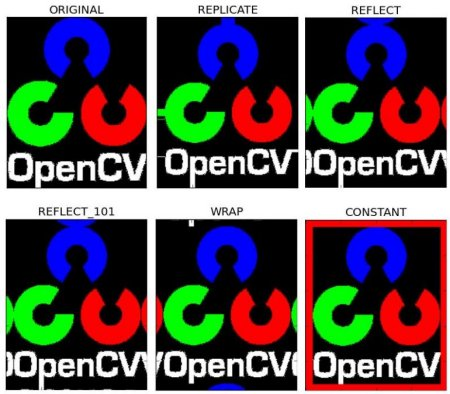
\includegraphics{./images/border.jpg}

    \subsubsection{2.2 Arithmetic Operations on
Images}\label{arithmetic-operations-on-images}

\textbf{Goals}

\begin{itemize}
\item
  Learn several arithmetic operations on images like addition,
  subtraction, bitwise operations etc.
\item
  You will learn these functions : cv2.add(), cv2.addWeighted() etc.
\end{itemize}

    \begin{Verbatim}[commandchars=\\\{\}]
{\color{incolor}In [{\color{incolor}47}]:} \PY{c+c1}{\PYZsh{} Image Addition \PYZhy{} 颜色上的叠加}
         \PY{c+c1}{\PYZsh{} OpenCV addition is a saturated operation while Numpy addition is a modulo operation}
         \PY{n}{x} \PY{o}{=} \PY{n}{np}\PY{o}{.}\PY{n}{uint8}\PY{p}{(}\PY{p}{[}\PY{l+m+mi}{250}\PY{p}{]}\PY{p}{)}
         \PY{n}{y} \PY{o}{=} \PY{n}{np}\PY{o}{.}\PY{n}{uint8}\PY{p}{(}\PY{p}{[}\PY{l+m+mi}{10}\PY{p}{]}\PY{p}{)}
         \PY{n+nb}{print}\PY{p}{(}\PY{n}{cv2}\PY{o}{.}\PY{n}{add}\PY{p}{(}\PY{n}{x}\PY{p}{,} \PY{n}{y}\PY{p}{)}\PY{p}{)}  \PY{c+c1}{\PYZsh{} 250+10 = 260 =\PYZgt{} 255}
         \PY{n+nb}{print}\PY{p}{(}\PY{n}{x} \PY{o}{+} \PY{n}{y}\PY{p}{)}          \PY{c+c1}{\PYZsh{} 250+10 = 260 \PYZpc{} 256 = 4}
\end{Verbatim}


    \begin{Verbatim}[commandchars=\\\{\}]
[[255]]
[4]

    \end{Verbatim}

    \begin{Verbatim}[commandchars=\\\{\}]
{\color{incolor}In [{\color{incolor}50}]:} \PY{c+c1}{\PYZsh{} Image Blending \PYZhy{} 颜色上的加权叠加 类似水印}
         \PY{c+c1}{\PYZsh{} Another image addition, but different weights are given to images, giving a feeling of blending or transparency}
         \PY{c+c1}{\PYZsh{} Images are added as per the equation: g(x) = alpha * f0(x) + beta * f1(x) + gamma}
         \PY{n}{img1} \PY{o}{=} \PY{n}{cv2}\PY{o}{.}\PY{n}{imread}\PY{p}{(}\PY{l+s+s1}{\PYZsq{}}\PY{l+s+s1}{./images/2.2\PYZus{}1.jpg}\PY{l+s+s1}{\PYZsq{}}\PY{p}{)}
         \PY{n}{img2} \PY{o}{=} \PY{n}{cv2}\PY{o}{.}\PY{n}{imread}\PY{p}{(}\PY{l+s+s1}{\PYZsq{}}\PY{l+s+s1}{./images/2.2\PYZus{}2.jpg}\PY{l+s+s1}{\PYZsq{}}\PY{p}{)}
         \PY{n}{img3} \PY{o}{=} \PY{n}{cv2}\PY{o}{.}\PY{n}{addWeighted}\PY{p}{(}\PY{n}{img1}\PY{p}{,} \PY{l+m+mf}{0.3}\PY{p}{,} \PY{n}{img2}\PY{p}{,} \PY{l+m+mf}{0.7}\PY{p}{,} \PY{l+m+mi}{0}\PY{p}{)}
         \PY{n}{plt}\PY{o}{.}\PY{n}{subplot}\PY{p}{(}\PY{l+m+mi}{131}\PY{p}{)}\PY{p}{,}\PY{n}{plt}\PY{o}{.}\PY{n}{imshow}\PY{p}{(}\PY{n}{img1}\PY{p}{,} \PY{l+s+s1}{\PYZsq{}}\PY{l+s+s1}{gray}\PY{l+s+s1}{\PYZsq{}}\PY{p}{)}
         \PY{n}{plt}\PY{o}{.}\PY{n}{subplot}\PY{p}{(}\PY{l+m+mi}{132}\PY{p}{)}\PY{p}{,}\PY{n}{plt}\PY{o}{.}\PY{n}{imshow}\PY{p}{(}\PY{n}{img2}\PY{p}{,} \PY{l+s+s1}{\PYZsq{}}\PY{l+s+s1}{gray}\PY{l+s+s1}{\PYZsq{}}\PY{p}{)}
         \PY{n}{plt}\PY{o}{.}\PY{n}{subplot}\PY{p}{(}\PY{l+m+mi}{133}\PY{p}{)}\PY{p}{,}\PY{n}{plt}\PY{o}{.}\PY{n}{imshow}\PY{p}{(}\PY{n}{img3}\PY{p}{,} \PY{l+s+s1}{\PYZsq{}}\PY{l+s+s1}{gray}\PY{l+s+s1}{\PYZsq{}}\PY{p}{)}
         \PY{n}{plt}\PY{o}{.}\PY{n}{show}\PY{p}{(}\PY{p}{)}
\end{Verbatim}


    \begin{center}
    \adjustimage{max size={0.9\linewidth}{0.9\paperheight}}{output_22_0.png}
    \end{center}
    { \hspace*{\fill} \\}
    
    \begin{Verbatim}[commandchars=\\\{\}]
{\color{incolor}In [{\color{incolor}51}]:} \PY{c+c1}{\PYZsh{} Bitwise Operations \PYZhy{} 图片上的覆盖等 类似透明度为0的水印}
         \PY{c+c1}{\PYZsh{} This includes bitwise AND, OR, NOT and XOR operations}
\end{Verbatim}


    \subsubsection{2.3 Performance Measurement and Improvement
Techniques}\label{performance-measurement-and-improvement-techniques}

\textbf{Goals}

\begin{itemize}
\item
  To measure the performance of your code.
\item
  Some tips to improve the performance of your code.
\item
  You will see these functions : cv2.getTickCount, cv2.getTickFrequency
  etc.
\end{itemize}

    \subsubsection{2.4 Mathematical Tools in
OpenCV}\label{mathematical-tools-in-opencv}

    \subsection{3. Image Processing in
OpenCV}\label{image-processing-in-opencv}

    \begin{Verbatim}[commandchars=\\\{\}]
{\color{incolor}In [{\color{incolor}2}]:} \PY{k+kn}{import} \PY{n+nn}{numpy} \PY{k}{as} \PY{n+nn}{np}
        \PY{k+kn}{import} \PY{n+nn}{cv2}
        \PY{k+kn}{from} \PY{n+nn}{matplotlib} \PY{k}{import} \PY{n}{pyplot} \PY{k}{as} \PY{n}{plt}
\end{Verbatim}


    \subsubsection{3.1 Changing Colorspaces}\label{changing-colorspaces}

\textbf{Goals}

\begin{itemize}
\item
  Learn how to convert images from one color-space to another, like BGR
  \textless{}-\/-\textgreater{} Gray, BGR \textless{}-\/-\textgreater{}
  HSV etc.
\item
  Create an application which extracts a colored object in a video
\item
  Learn following functions : cv2.cvtColor(), cv2.inRange() etc.
\end{itemize}

    \begin{Verbatim}[commandchars=\\\{\}]
{\color{incolor}In [{\color{incolor}3}]:} \PY{c+c1}{\PYZsh{} There are more than 150 color\PYZhy{}space conversion methods available in OpenCV}
        \PY{n}{colors} \PY{o}{=} \PY{p}{[}\PY{n}{x} \PY{k}{for} \PY{n}{x} \PY{o+ow}{in} \PY{n+nb}{dir}\PY{p}{(}\PY{n}{cv2}\PY{p}{)} \PY{k}{if} \PY{n}{x}\PY{o}{.}\PY{n}{startswith}\PY{p}{(}\PY{l+s+s1}{\PYZsq{}}\PY{l+s+s1}{COLOR\PYZus{}}\PY{l+s+s1}{\PYZsq{}}\PY{p}{)}\PY{p}{]}
\end{Verbatim}


    cv2.cvtColor(input\_image,
flag),其中flag=cv2.COLOR\_BGR2GRAY/cv2.COLOR\_BGR2HSV

    \begin{Verbatim}[commandchars=\\\{\}]
{\color{incolor}In [{\color{incolor}56}]:} \PY{c+c1}{\PYZsh{} Find the HSV value of BGR}
         \PY{n}{green} \PY{o}{=} \PY{n}{np}\PY{o}{.}\PY{n}{uint8}\PY{p}{(}\PY{p}{[}\PY{p}{[}\PY{p}{[}\PY{l+m+mi}{0}\PY{p}{,} \PY{l+m+mi}{255}\PY{p}{,} \PY{l+m+mi}{0}\PY{p}{]}\PY{p}{]}\PY{p}{]}\PY{p}{)}    \PY{c+c1}{\PYZsh{}注意,3层中括号\PYZhy{}\PYZhy{}3维,图片表示形式}
         \PY{n+nb}{print}\PY{p}{(}\PY{n}{cv2}\PY{o}{.}\PY{n}{cvtColor}\PY{p}{(}\PY{n}{green}\PY{p}{,} \PY{n}{cv2}\PY{o}{.}\PY{n}{COLOR\PYZus{}BGR2HSV}\PY{p}{)}\PY{p}{)}
\end{Verbatim}


    \begin{Verbatim}[commandchars=\\\{\}]
[[[ 60 255 255]]]

    \end{Verbatim}

    \subsubsection{3.2 Geometric Transformations of
Images}\label{geometric-transformations-of-images}

\textbf{Goals}

\begin{itemize}
\item
  Learn to apply different geometric transformation to images like
  translation, rotation, affine transformation etc.
\item
  Learn these functions: cv2.resize, cv2.warpAffine,
  cv2.warpPerspective, cv2.getPerspectiveTransform
\end{itemize}

    \begin{Verbatim}[commandchars=\\\{\}]
{\color{incolor}In [{\color{incolor}57}]:} \PY{c+c1}{\PYZsh{} Scaling}
         
         \PY{c+c1}{\PYZsh{} Shifting}
         
         \PY{c+c1}{\PYZsh{} Rotation}
\end{Verbatim}


    \begin{Verbatim}[commandchars=\\\{\}]
{\color{incolor}In [{\color{incolor}58}]:} \PY{c+c1}{\PYZsh{} Affine Transformation: 把原图中指定的3个点,通过各种操作Transform到新的3个位置,原图平行结构不变,只是视角变化}
\end{Verbatim}


    \begin{figure}
\centering
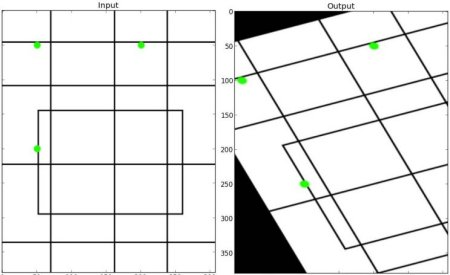
\includegraphics{./images/3.2_1.jpg}
\caption{avatar}
\end{figure}

    \begin{Verbatim}[commandchars=\\\{\}]
{\color{incolor}In [{\color{incolor}59}]:} \PY{c+c1}{\PYZsh{} Perspective Transformation: 把原图中指定的4个点,通过各种操作Transform到新的4个位置. 下图是梯形\PYZhy{}\PYZhy{}\PYZgt{}矩形}
\end{Verbatim}


    \begin{figure}
\centering
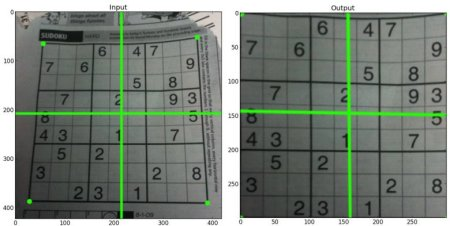
\includegraphics{./images/3.2_2.jpg}
\caption{avatar}
\end{figure}

    \subsubsection{3.3 Image Thresholding}\label{image-thresholding}

\textbf{Goals}

\begin{itemize}
\item
  Learn Simple thresholding, Adaptive thresholding, Otsu's thresholding
  etc.
\item
  Learn these functions : cv2.threshold, cv2.adaptiveThreshold etc.
\end{itemize}

    \begin{Verbatim}[commandchars=\\\{\}]
{\color{incolor}In [{\color{incolor} }]:} \PY{c+c1}{\PYZsh{} Simple Thresholdinn: 全局阈值 类似于图片二值化}
        \PY{n}{img} \PY{o}{=} \PY{n}{cv2}\PY{o}{.}\PY{n}{imread}\PY{p}{(}\PY{l+s+s1}{\PYZsq{}}\PY{l+s+s1}{gradient.png}\PY{l+s+s1}{\PYZsq{}}\PY{p}{,}\PY{l+m+mi}{0}\PY{p}{)}
        \PY{n}{ret}\PY{p}{,}\PY{n}{thresh1} \PY{o}{=} \PY{n}{cv2}\PY{o}{.}\PY{n}{threshold}\PY{p}{(}\PY{n}{img}\PY{p}{,}\PY{l+m+mi}{127}\PY{p}{,}\PY{l+m+mi}{255}\PY{p}{,}\PY{n}{cv2}\PY{o}{.}\PY{n}{THRESH\PYZus{}BINARY}\PY{p}{)}
        \PY{n}{ret}\PY{p}{,}\PY{n}{thresh2} \PY{o}{=} \PY{n}{cv2}\PY{o}{.}\PY{n}{threshold}\PY{p}{(}\PY{n}{img}\PY{p}{,}\PY{l+m+mi}{127}\PY{p}{,}\PY{l+m+mi}{255}\PY{p}{,}\PY{n}{cv2}\PY{o}{.}\PY{n}{THRESH\PYZus{}BINARY\PYZus{}INV}\PY{p}{)}
        \PY{n}{ret}\PY{p}{,}\PY{n}{thresh3} \PY{o}{=} \PY{n}{cv2}\PY{o}{.}\PY{n}{threshold}\PY{p}{(}\PY{n}{img}\PY{p}{,}\PY{l+m+mi}{127}\PY{p}{,}\PY{l+m+mi}{255}\PY{p}{,}\PY{n}{cv2}\PY{o}{.}\PY{n}{THRESH\PYZus{}TRUNC}\PY{p}{)}
        \PY{n}{ret}\PY{p}{,}\PY{n}{thresh4} \PY{o}{=} \PY{n}{cv2}\PY{o}{.}\PY{n}{threshold}\PY{p}{(}\PY{n}{img}\PY{p}{,}\PY{l+m+mi}{127}\PY{p}{,}\PY{l+m+mi}{255}\PY{p}{,}\PY{n}{cv2}\PY{o}{.}\PY{n}{THRESH\PYZus{}TOZERO}\PY{p}{)}
        \PY{n}{ret}\PY{p}{,}\PY{n}{thresh5} \PY{o}{=} \PY{n}{cv2}\PY{o}{.}\PY{n}{threshold}\PY{p}{(}\PY{n}{img}\PY{p}{,}\PY{l+m+mi}{127}\PY{p}{,}\PY{l+m+mi}{255}\PY{p}{,}\PY{n}{cv2}\PY{o}{.}\PY{n}{THRESH\PYZus{}TOZERO\PYZus{}INV}\PY{p}{)}
\end{Verbatim}


    运行结果: 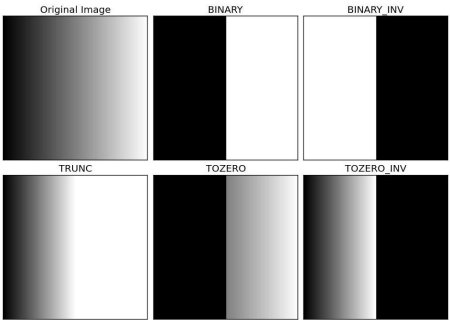
\includegraphics{./images/3.3_1.jpg}

    \begin{Verbatim}[commandchars=\\\{\}]
{\color{incolor}In [{\color{incolor}60}]:} \PY{c+c1}{\PYZsh{} Adaptive Thresholding: 局部阈值  局部均值或加权和}
         \PY{c+c1}{\PYZsh{} Algorithm calculates threshold for a small regions of image to get different thresholds for different regions, }
         \PY{c+c1}{\PYZsh{} giving us better results for images with varying illumination}
\end{Verbatim}


    \begin{figure}
\centering
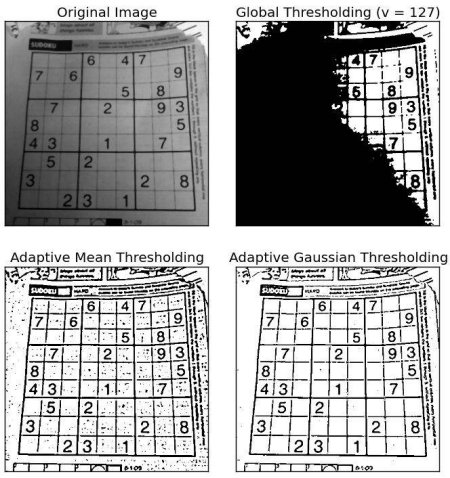
\includegraphics{./images/3.3_2.jpg}
\caption{avatar}
\end{figure}

    \begin{Verbatim}[commandchars=\\\{\}]
{\color{incolor}In [{\color{incolor}61}]:} \PY{c+c1}{\PYZsh{} Otsu\PYZsq{}s Binarization: 待看!?}
\end{Verbatim}


    \begin{figure}
\centering
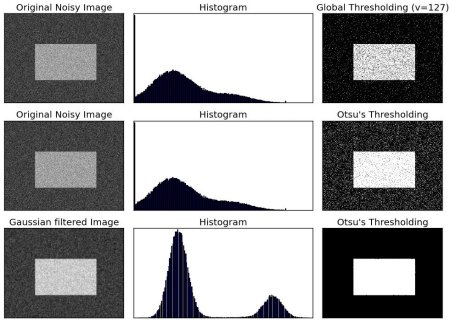
\includegraphics{./images/3.3_3.jpg}
\caption{avatar}
\end{figure}

    \subsubsection{3.4 Smoothing Images}\label{smoothing-images}

\textbf{Goals}

\begin{itemize}
\item
  Blur the images with various low pass filters
\item
  Apply custom-made filters to images (2D convolution)
\end{itemize}

    \begin{Verbatim}[commandchars=\\\{\}]
{\color{incolor}In [{\color{incolor}9}]:} \PY{c+c1}{\PYZsh{} 2D Convolution (Image Filtering) \PYZhy{} 卷积}
        \PY{c+c1}{\PYZsh{} Low\PYZhy{}pass  filters(LPF) helps in removing noises, blurring the images etc.}
        \PY{c+c1}{\PYZsh{} High\PYZhy{}pass filters(HPF) helps in finding edges in the images.}
        \PY{n}{img} \PY{o}{=} \PY{n}{cv2}\PY{o}{.}\PY{n}{imread}\PY{p}{(}\PY{l+s+s1}{\PYZsq{}}\PY{l+s+s1}{./images/opencv\PYZhy{}logo.png}\PY{l+s+s1}{\PYZsq{}}\PY{p}{)}
        
        \PY{n}{kernel} \PY{o}{=} \PY{n}{np}\PY{o}{.}\PY{n}{ones}\PY{p}{(}\PY{p}{(}\PY{l+m+mi}{7}\PY{p}{,}\PY{l+m+mi}{7}\PY{p}{)}\PY{p}{,}\PY{n}{np}\PY{o}{.}\PY{n}{float32}\PY{p}{)}\PY{o}{/}\PY{l+m+mi}{49}
        \PY{n}{dst} \PY{o}{=} \PY{n}{cv2}\PY{o}{.}\PY{n}{filter2D}\PY{p}{(}\PY{n}{img} \PY{p}{,}\PY{o}{\PYZhy{}}\PY{l+m+mi}{1}\PY{p}{,} \PY{n}{kernel}\PY{p}{)}   \PY{c+c1}{\PYZsh{} The function does actually compute correlation, not convolution}
        
        \PY{n}{plt}\PY{o}{.}\PY{n}{subplot}\PY{p}{(}\PY{l+m+mi}{121}\PY{p}{)}\PY{p}{,}\PY{n}{plt}\PY{o}{.}\PY{n}{imshow}\PY{p}{(}\PY{n}{img}\PY{p}{)}\PY{p}{,}\PY{n}{plt}\PY{o}{.}\PY{n}{title}\PY{p}{(}\PY{l+s+s1}{\PYZsq{}}\PY{l+s+s1}{Original}\PY{l+s+s1}{\PYZsq{}}\PY{p}{)}
        \PY{n}{plt}\PY{o}{.}\PY{n}{xticks}\PY{p}{(}\PY{p}{[}\PY{p}{]}\PY{p}{)}\PY{p}{,} \PY{n}{plt}\PY{o}{.}\PY{n}{yticks}\PY{p}{(}\PY{p}{[}\PY{p}{]}\PY{p}{)}
        \PY{n}{plt}\PY{o}{.}\PY{n}{subplot}\PY{p}{(}\PY{l+m+mi}{122}\PY{p}{)}\PY{p}{,}\PY{n}{plt}\PY{o}{.}\PY{n}{imshow}\PY{p}{(}\PY{n}{dst}\PY{p}{)}\PY{p}{,}\PY{n}{plt}\PY{o}{.}\PY{n}{title}\PY{p}{(}\PY{l+s+s1}{\PYZsq{}}\PY{l+s+s1}{Averaging}\PY{l+s+s1}{\PYZsq{}}\PY{p}{)}
        \PY{n}{plt}\PY{o}{.}\PY{n}{xticks}\PY{p}{(}\PY{p}{[}\PY{p}{]}\PY{p}{)}\PY{p}{,} \PY{n}{plt}\PY{o}{.}\PY{n}{yticks}\PY{p}{(}\PY{p}{[}\PY{p}{]}\PY{p}{)}
        \PY{n}{plt}\PY{o}{.}\PY{n}{show}\PY{p}{(}\PY{p}{)}
\end{Verbatim}


    \begin{center}
    \adjustimage{max size={0.9\linewidth}{0.9\paperheight}}{output_46_0.png}
    \end{center}
    { \hspace*{\fill} \\}
    
    \begin{Verbatim}[commandchars=\\\{\}]
{\color{incolor}In [{\color{incolor} }]:} \PY{c+c1}{\PYZsh{} Image Blurring (Image Smoothing) \PYZhy{} 4 types of blurring techniques}
        \PY{c+c1}{\PYZsh{} Averaging}
        \PY{n}{blur} \PY{o}{=} \PY{n}{cv2}\PY{o}{.}\PY{n}{blur}\PY{p}{(}\PY{n}{img}\PY{p}{,}\PY{p}{(}\PY{l+m+mi}{5}\PY{p}{,}\PY{l+m+mi}{5}\PY{p}{)}\PY{p}{)}
        \PY{c+c1}{\PYZsh{} Gaussian Blurring}
        \PY{n}{blur} \PY{o}{=} \PY{n}{cv2}\PY{o}{.}\PY{n}{GaussianBlur}\PY{p}{(}\PY{n}{img}\PY{p}{,}\PY{p}{(}\PY{l+m+mi}{5}\PY{p}{,}\PY{l+m+mi}{5}\PY{p}{)}\PY{p}{,}\PY{l+m+mi}{0}\PY{p}{)}
        \PY{c+c1}{\PYZsh{} Median Blurring}
        \PY{n}{median} \PY{o}{=} \PY{n}{cv2}\PY{o}{.}\PY{n}{medianBlur}\PY{p}{(}\PY{n}{img}\PY{p}{,}\PY{l+m+mi}{5}\PY{p}{)}
        \PY{c+c1}{\PYZsh{} Bilateral Filtering}
        \PY{n}{blur} \PY{o}{=} \PY{n}{cv2}\PY{o}{.}\PY{n}{bilateralFilter}\PY{p}{(}\PY{n}{img}\PY{p}{,}\PY{l+m+mi}{9}\PY{p}{,}\PY{l+m+mi}{75}\PY{p}{,}\PY{l+m+mi}{75}\PY{p}{)}
\end{Verbatim}


    \subsubsection{3.5 Morphological
Transformations}\label{morphological-transformations}

\textbf{Goals}

\begin{itemize}
\item
  We will learn different morphological operations like Erosion,
  Dilation, Opening, Closing etc.
\item
  We will see different functions like : cv2.erode(), cv2.dilate(),
  cv2.morphologyEx() etc.
\end{itemize}

    \begin{Verbatim}[commandchars=\\\{\}]
{\color{incolor}In [{\color{incolor}16}]:} \PY{n}{img} \PY{o}{=} \PY{n}{cv2}\PY{o}{.}\PY{n}{imread}\PY{p}{(}\PY{l+s+s1}{\PYZsq{}}\PY{l+s+s1}{./images/j.png}\PY{l+s+s1}{\PYZsq{}}\PY{p}{,} \PY{l+m+mi}{1}\PY{p}{)}
         \PY{n}{img} \PY{o}{=} \PY{n}{img}\PY{p}{[}\PY{p}{:}\PY{p}{,} \PY{p}{:}\PY{p}{,} \PY{p}{:}\PY{p}{:}\PY{o}{\PYZhy{}}\PY{l+m+mi}{1}\PY{p}{]}
         \PY{n}{kernel} \PY{o}{=} \PY{n}{np}\PY{o}{.}\PY{n}{ones}\PY{p}{(}\PY{p}{(}\PY{l+m+mi}{5}\PY{p}{,}\PY{l+m+mi}{5}\PY{p}{)}\PY{p}{,}\PY{n}{np}\PY{o}{.}\PY{n}{uint8}\PY{p}{)}
         
         \PY{n}{erosion}  \PY{o}{=} \PY{n}{cv2}\PY{o}{.}\PY{n}{erode}\PY{p}{(}\PY{n}{img}\PY{p}{,} \PY{n}{kernel}\PY{p}{,} \PY{n}{iterations}\PY{o}{=}\PY{l+m+mi}{1}\PY{p}{)}
         \PY{n}{dilation} \PY{o}{=} \PY{n}{cv2}\PY{o}{.}\PY{n}{dilate}\PY{p}{(}\PY{n}{img}\PY{p}{,} \PY{n}{kernel}\PY{p}{,} \PY{n}{iterations}\PY{o}{=}\PY{l+m+mi}{1}\PY{p}{)}
         \PY{n}{opening}  \PY{o}{=} \PY{n}{cv2}\PY{o}{.}\PY{n}{morphologyEx}\PY{p}{(}\PY{n}{img}\PY{p}{,} \PY{n}{cv2}\PY{o}{.}\PY{n}{MORPH\PYZus{}OPEN}\PY{p}{,}     \PY{n}{kernel}\PY{p}{)} \PY{c+c1}{\PYZsh{} =Erosion followed by dilation. Useful in removing noise}
         \PY{n}{closing}  \PY{o}{=} \PY{n}{cv2}\PY{o}{.}\PY{n}{morphologyEx}\PY{p}{(}\PY{n}{img}\PY{p}{,} \PY{n}{cv2}\PY{o}{.}\PY{n}{MORPH\PYZus{}CLOSE}\PY{p}{,}    \PY{n}{kernel}\PY{p}{)} \PY{c+c1}{\PYZsh{} =Dilation followed by erosion. Useful in closing small holes or small black points}
         \PY{n}{gradient} \PY{o}{=} \PY{n}{cv2}\PY{o}{.}\PY{n}{morphologyEx}\PY{p}{(}\PY{n}{img}\PY{p}{,} \PY{n}{cv2}\PY{o}{.}\PY{n}{MORPH\PYZus{}GRADIENT}\PY{p}{,} \PY{n}{kernel}\PY{p}{)}
         \PY{n}{tophat}   \PY{o}{=} \PY{n}{cv2}\PY{o}{.}\PY{n}{morphologyEx}\PY{p}{(}\PY{n}{img}\PY{p}{,} \PY{n}{cv2}\PY{o}{.}\PY{n}{MORPH\PYZus{}TOPHAT}\PY{p}{,}   \PY{n}{kernel}\PY{p}{)}
         \PY{n}{blackhat} \PY{o}{=} \PY{n}{cv2}\PY{o}{.}\PY{n}{morphologyEx}\PY{p}{(}\PY{n}{img}\PY{p}{,} \PY{n}{cv2}\PY{o}{.}\PY{n}{MORPH\PYZus{}BLACKHAT}\PY{p}{,} \PY{n}{kernel}\PY{p}{)}
         
         \PY{n}{plt}\PY{o}{.}\PY{n}{subplot}\PY{p}{(}\PY{l+m+mi}{231}\PY{p}{)}\PY{p}{,} \PY{n}{plt}\PY{o}{.}\PY{n}{imshow}\PY{p}{(}\PY{n}{img}\PY{p}{)}\PY{p}{,} \PY{n}{plt}\PY{o}{.}\PY{n}{title}\PY{p}{(}\PY{l+s+s1}{\PYZsq{}}\PY{l+s+s1}{Original}\PY{l+s+s1}{\PYZsq{}}\PY{p}{)}\PY{p}{,} \PY{n}{plt}\PY{o}{.}\PY{n}{xticks}\PY{p}{(}\PY{p}{[}\PY{p}{]}\PY{p}{)}\PY{p}{,} \PY{n}{plt}\PY{o}{.}\PY{n}{yticks}\PY{p}{(}\PY{p}{[}\PY{p}{]}\PY{p}{)}
         \PY{n}{plt}\PY{o}{.}\PY{n}{subplot}\PY{p}{(}\PY{l+m+mi}{232}\PY{p}{)}\PY{p}{,}\PY{n}{plt}\PY{o}{.}\PY{n}{imshow}\PY{p}{(}\PY{n}{erosion}\PY{p}{)}\PY{p}{,}\PY{n}{plt}\PY{o}{.}\PY{n}{title}\PY{p}{(}\PY{l+s+s1}{\PYZsq{}}\PY{l+s+s1}{Erosion}\PY{l+s+s1}{\PYZsq{}}\PY{p}{)}\PY{p}{,} \PY{n}{plt}\PY{o}{.}\PY{n}{xticks}\PY{p}{(}\PY{p}{[}\PY{p}{]}\PY{p}{)}\PY{p}{,} \PY{n}{plt}\PY{o}{.}\PY{n}{yticks}\PY{p}{(}\PY{p}{[}\PY{p}{]}\PY{p}{)}
         \PY{n}{plt}\PY{o}{.}\PY{n}{subplot}\PY{p}{(}\PY{l+m+mi}{233}\PY{p}{)}\PY{p}{,}\PY{n}{plt}\PY{o}{.}\PY{n}{imshow}\PY{p}{(}\PY{n}{dilation}\PY{p}{)}\PY{p}{,}\PY{n}{plt}\PY{o}{.}\PY{n}{title}\PY{p}{(}\PY{l+s+s1}{\PYZsq{}}\PY{l+s+s1}{Dilation}\PY{l+s+s1}{\PYZsq{}}\PY{p}{)}\PY{p}{,} \PY{n}{plt}\PY{o}{.}\PY{n}{xticks}\PY{p}{(}\PY{p}{[}\PY{p}{]}\PY{p}{)}\PY{p}{,} \PY{n}{plt}\PY{o}{.}\PY{n}{yticks}\PY{p}{(}\PY{p}{[}\PY{p}{]}\PY{p}{)}
         \PY{n}{plt}\PY{o}{.}\PY{n}{subplot}\PY{p}{(}\PY{l+m+mi}{234}\PY{p}{)}\PY{p}{,}\PY{n}{plt}\PY{o}{.}\PY{n}{imshow}\PY{p}{(}\PY{n}{gradient}\PY{p}{)}\PY{p}{,}\PY{n}{plt}\PY{o}{.}\PY{n}{title}\PY{p}{(}\PY{l+s+s1}{\PYZsq{}}\PY{l+s+s1}{Gradient}\PY{l+s+s1}{\PYZsq{}}\PY{p}{)}\PY{p}{,} \PY{n}{plt}\PY{o}{.}\PY{n}{xticks}\PY{p}{(}\PY{p}{[}\PY{p}{]}\PY{p}{)}\PY{p}{,} \PY{n}{plt}\PY{o}{.}\PY{n}{yticks}\PY{p}{(}\PY{p}{[}\PY{p}{]}\PY{p}{)}
         \PY{n}{plt}\PY{o}{.}\PY{n}{subplot}\PY{p}{(}\PY{l+m+mi}{235}\PY{p}{)}\PY{p}{,}\PY{n}{plt}\PY{o}{.}\PY{n}{imshow}\PY{p}{(}\PY{n}{tophat}\PY{p}{)}\PY{p}{,}\PY{n}{plt}\PY{o}{.}\PY{n}{title}\PY{p}{(}\PY{l+s+s1}{\PYZsq{}}\PY{l+s+s1}{Tophat}\PY{l+s+s1}{\PYZsq{}}\PY{p}{)}\PY{p}{,} \PY{n}{plt}\PY{o}{.}\PY{n}{xticks}\PY{p}{(}\PY{p}{[}\PY{p}{]}\PY{p}{)}\PY{p}{,} \PY{n}{plt}\PY{o}{.}\PY{n}{yticks}\PY{p}{(}\PY{p}{[}\PY{p}{]}\PY{p}{)}
         \PY{n}{plt}\PY{o}{.}\PY{n}{subplot}\PY{p}{(}\PY{l+m+mi}{236}\PY{p}{)}\PY{p}{,}\PY{n}{plt}\PY{o}{.}\PY{n}{imshow}\PY{p}{(}\PY{n}{blackhat}\PY{p}{)}\PY{p}{,}\PY{n}{plt}\PY{o}{.}\PY{n}{title}\PY{p}{(}\PY{l+s+s1}{\PYZsq{}}\PY{l+s+s1}{Blackhat}\PY{l+s+s1}{\PYZsq{}}\PY{p}{)}\PY{p}{,} \PY{n}{plt}\PY{o}{.}\PY{n}{xticks}\PY{p}{(}\PY{p}{[}\PY{p}{]}\PY{p}{)}\PY{p}{,} \PY{n}{plt}\PY{o}{.}\PY{n}{yticks}\PY{p}{(}\PY{p}{[}\PY{p}{]}\PY{p}{)}
         \PY{n}{plt}\PY{o}{.}\PY{n}{show}\PY{p}{(}\PY{p}{)}
\end{Verbatim}


    \begin{center}
    \adjustimage{max size={0.9\linewidth}{0.9\paperheight}}{output_49_0.png}
    \end{center}
    { \hspace*{\fill} \\}
    
    \begin{Verbatim}[commandchars=\\\{\}]
{\color{incolor}In [{\color{incolor}17}]:} \PY{c+c1}{\PYZsh{} Get Structuring Element.\PYZhy{} Just pass the shape and size of the kernel, you get the desired kernel.}
         \PY{n+nb}{print}\PY{p}{(}\PY{n}{cv2}\PY{o}{.}\PY{n}{getStructuringElement}\PY{p}{(}\PY{n}{cv2}\PY{o}{.}\PY{n}{MORPH\PYZus{}RECT}\PY{p}{,}    \PY{p}{(}\PY{l+m+mi}{5}\PY{p}{,}\PY{l+m+mi}{5}\PY{p}{)}\PY{p}{)}\PY{p}{)}
         \PY{n+nb}{print}\PY{p}{(}\PY{n}{cv2}\PY{o}{.}\PY{n}{getStructuringElement}\PY{p}{(}\PY{n}{cv2}\PY{o}{.}\PY{n}{MORPH\PYZus{}ELLIPSE}\PY{p}{,} \PY{p}{(}\PY{l+m+mi}{5}\PY{p}{,}\PY{l+m+mi}{5}\PY{p}{)}\PY{p}{)}\PY{p}{)}
         \PY{n+nb}{print}\PY{p}{(}\PY{n}{cv2}\PY{o}{.}\PY{n}{getStructuringElement}\PY{p}{(}\PY{n}{cv2}\PY{o}{.}\PY{n}{MORPH\PYZus{}CROSS}\PY{p}{,}   \PY{p}{(}\PY{l+m+mi}{5}\PY{p}{,}\PY{l+m+mi}{5}\PY{p}{)}\PY{p}{)}\PY{p}{)}
\end{Verbatim}


    \begin{Verbatim}[commandchars=\\\{\}]
[[1 1 1 1 1]
 [1 1 1 1 1]
 [1 1 1 1 1]
 [1 1 1 1 1]
 [1 1 1 1 1]]
[[0 0 1 0 0]
 [1 1 1 1 1]
 [1 1 1 1 1]
 [1 1 1 1 1]
 [0 0 1 0 0]]
[[0 0 1 0 0]
 [0 0 1 0 0]
 [1 1 1 1 1]
 [0 0 1 0 0]
 [0 0 1 0 0]]

    \end{Verbatim}

    \subsubsection{3.6 Image Gradients}\label{image-gradients}

\textbf{Goals}

\begin{itemize}
\item
  Find Image gradients, edges etc
\item
  We will see following functions : cv2.Sobel(), cv2.Scharr(),
  cv2.Laplacian() etc
\end{itemize}

    \begin{Verbatim}[commandchars=\\\{\}]
{\color{incolor}In [{\color{incolor} }]:} \PY{n}{img} \PY{o}{=} \PY{n}{cv2}\PY{o}{.}\PY{n}{imread}\PY{p}{(}\PY{l+s+s1}{\PYZsq{}}\PY{l+s+s1}{dave.jpg}\PY{l+s+s1}{\PYZsq{}}\PY{p}{,}\PY{l+m+mi}{0}\PY{p}{)}
        
        \PY{n}{laplacian} \PY{o}{=} \PY{n}{cv2}\PY{o}{.}\PY{n}{Laplacian}\PY{p}{(}\PY{n}{img}\PY{p}{,}\PY{n}{cv2}\PY{o}{.}\PY{n}{CV\PYZus{}64F}\PY{p}{)}
        \PY{n}{sobelx} \PY{o}{=} \PY{n}{cv2}\PY{o}{.}\PY{n}{Sobel}\PY{p}{(}\PY{n}{img}\PY{p}{,}\PY{n}{cv2}\PY{o}{.}\PY{n}{CV\PYZus{}64F}\PY{p}{,}\PY{l+m+mi}{1}\PY{p}{,}\PY{l+m+mi}{0}\PY{p}{,}\PY{n}{ksize}\PY{o}{=}\PY{l+m+mi}{5}\PY{p}{)}
        \PY{n}{sobely} \PY{o}{=} \PY{n}{cv2}\PY{o}{.}\PY{n}{Sobel}\PY{p}{(}\PY{n}{img}\PY{p}{,}\PY{n}{cv2}\PY{o}{.}\PY{n}{CV\PYZus{}64F}\PY{p}{,}\PY{l+m+mi}{0}\PY{p}{,}\PY{l+m+mi}{1}\PY{p}{,}\PY{n}{ksize}\PY{o}{=}\PY{l+m+mi}{5}\PY{p}{)}
\end{Verbatim}


    Result: 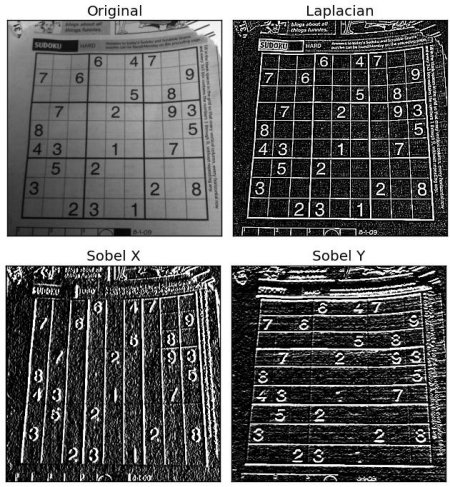
\includegraphics{./images/3.6_1.jpg}

    \subsubsection{3.7 Canny Edge Detection}\label{canny-edge-detection}

\textbf{Goals}

\begin{itemize}
\item
  Concept of Canny edge detection
\item
  OpenCV functions for that : cv2.Canny()
\end{itemize}

    \begin{Verbatim}[commandchars=\\\{\}]
{\color{incolor}In [{\color{incolor} }]:} \PY{n}{img} \PY{o}{=} \PY{n}{cv2}\PY{o}{.}\PY{n}{imread}\PY{p}{(}\PY{l+s+s1}{\PYZsq{}}\PY{l+s+s1}{messi5.jpg}\PY{l+s+s1}{\PYZsq{}}\PY{p}{,}\PY{l+m+mi}{0}\PY{p}{)}
        \PY{n}{edges} \PY{o}{=} \PY{n}{cv2}\PY{o}{.}\PY{n}{Canny}\PY{p}{(}\PY{n}{img}\PY{p}{,} \PY{n}{threshold1}\PY{o}{=}\PY{l+m+mi}{100}\PY{p}{,} \PY{n}{threshold2}\PY{o}{=}\PY{l+m+mi}{200}\PY{p}{)}
\end{Verbatim}


    Result: 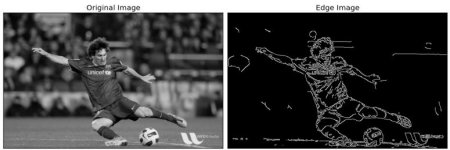
\includegraphics{./images/3.7_1.jpg}

    \subsubsection{3.8 Image Pyramids}\label{image-pyramids}

\textbf{Goals}

\begin{itemize}
\item
  We will learn about Image Pyramids
\item
  We will use Image pyramids to create a new fruit, ``Orapple''
\item
  We will see these functions: cv2.pyrUp(), cv2.pyrDown()
\end{itemize}

    \subsubsection{3.9 Contours in OpenCV}\label{contours-in-opencv}

\paragraph{3.9.1 Contours : Getting
Started}\label{contours-getting-started}

\textbf{Goals}

\begin{itemize}
\item
  Understand what contours are.
\item
  Learn to find contours, draw contours etc
\item
  You will see these functions : cv2.findContours(), cv2.drawContours()
\end{itemize}

    \paragraph{3.9.2 Contour Features}\label{contour-features}

\textbf{Goals}

\begin{itemize}
\tightlist
\item
  Find the different features of contours, like area, perimeter,
  centroid, bounding box etc
\end{itemize}

    \paragraph{3.9.3 Contour Properties}\label{contour-properties}

\textbf{Goals}

\begin{itemize}
\tightlist
\item
  Extract some frequently used properties of objects like Solidity,
  Equivalent Diameter, Mask image, Mean Intensity, Extrem points etc.
\end{itemize}

    \paragraph{3.9.4 Contours : More
Functions}\label{contours-more-functions}

\begin{itemize}
\item
  Learn about convexity defects and how to find them.
\item
  Find shortest distance from a point to a polygon.
\item
  Match different shapes.
\end{itemize}

    \paragraph{3.9.5 Contours Hierarchy}\label{contours-hierarchy}

\begin{itemize}
\tightlist
\item
  CLearn about the hierarchy of contours, i.e. the parent-child
  relationship in Contours.
\end{itemize}

    \subsubsection{3.10 Histograms in OpenCV}\label{histograms-in-opencv}

\textbf{Goals}

\begin{itemize}
\item
\end{itemize}

    \subsubsection{3.11 Image Transforms in
OpenCV}\label{image-transforms-in-opencv}

\paragraph{3.11.1 Fourier Transform}\label{fourier-transform}

\textbf{Goals}

\begin{itemize}
\item
  Find the Fourier Transform of images using OpenCV
\item
  utilize the FFT functions available in Numpy
\item
  Some applications of Fourier Transform
\item
  We will see following functions : cv2.dft(), cv2.idft() etc
\end{itemize}

    \subsubsection{3.12 Template Matching}\label{template-matching}

\textbf{Goals}

\begin{itemize}
\item
  Find objects in an image using Template Matching
\item
  You will see these functions : cv2.matchTemplate(), cv2.minMaxLoc()
\end{itemize}

    \subsubsection{3.13 Hough Line Transform}\label{hough-line-transform}

\textbf{Goals}

\begin{itemize}
\item
  We will understand the concept of Hough Tranform.
\item
  We will see how to use it detect lines in an image.
\item
  We will see following functions: cv2.HoughLines(), cv2.HoughLinesP()
\end{itemize}

\textbf{Theory}

Hough Transform is a popular technique to detect any shape, if you can
represent that shape in mathematical form. It can detect the shape even
if it is broken or distorted a little bit.

    \begin{Verbatim}[commandchars=\\\{\}]
{\color{incolor}In [{\color{incolor}39}]:} \PY{n}{img} \PY{o}{=} \PY{n}{cv2}\PY{o}{.}\PY{n}{imread}\PY{p}{(}\PY{l+s+s1}{\PYZsq{}}\PY{l+s+s1}{demo.jpg}\PY{l+s+s1}{\PYZsq{}}\PY{p}{)}
         \PY{n}{gray} \PY{o}{=} \PY{n}{cv2}\PY{o}{.}\PY{n}{cvtColor}\PY{p}{(}\PY{n}{img}\PY{p}{,} \PY{n}{cv2}\PY{o}{.}\PY{n}{COLOR\PYZus{}BGR2GRAY}\PY{p}{)}
         \PY{n}{edges} \PY{o}{=} \PY{n}{cv2}\PY{o}{.}\PY{n}{Canny}\PY{p}{(}\PY{n}{gray}\PY{p}{,} \PY{l+m+mi}{400}\PY{p}{,} \PY{l+m+mi}{500}\PY{p}{,} \PY{n}{apertureSize}\PY{o}{=}\PY{l+m+mi}{3}\PY{p}{)}
         
         \PY{c+c1}{\PYZsh{} Finds lines in a binary image using the standard Hough transform.}
         \PY{n}{img2} \PY{o}{=} \PY{n}{img}\PY{o}{.}\PY{n}{copy}\PY{p}{(}\PY{p}{)}
         \PY{n}{lines} \PY{o}{=} \PY{n}{cv2}\PY{o}{.}\PY{n}{HoughLines}\PY{p}{(}\PY{n}{image}\PY{o}{=}\PY{n}{edges}\PY{p}{,} \PY{n}{rho}\PY{o}{=}\PY{l+m+mi}{1}\PY{p}{,} \PY{n}{theta}\PY{o}{=}\PY{n}{np}\PY{o}{.}\PY{n}{pi}\PY{o}{/}\PY{l+m+mi}{180}\PY{p}{,} \PY{n}{threshold}\PY{o}{=}\PY{l+m+mi}{200}\PY{p}{)}
         \PY{k}{for} \PY{n}{rho}\PY{p}{,} \PY{n}{theta} \PY{o+ow}{in} \PY{n}{lines}\PY{p}{[}\PY{l+m+mi}{0}\PY{p}{]}\PY{p}{:}
             \PY{n}{a}\PY{p}{,} \PY{n}{b} \PY{o}{=} \PY{n}{np}\PY{o}{.}\PY{n}{cos}\PY{p}{(}\PY{n}{theta}\PY{p}{)}\PY{p}{,} \PY{n}{np}\PY{o}{.}\PY{n}{sin}\PY{p}{(}\PY{n}{theta}\PY{p}{)}
             \PY{n}{x0} \PY{o}{=} \PY{n}{a} \PY{o}{*} \PY{n}{rho}
             \PY{n}{y0} \PY{o}{=} \PY{n}{b} \PY{o}{*} \PY{n}{rho}
             \PY{n}{x1} \PY{o}{=} \PY{n+nb}{int}\PY{p}{(}\PY{n}{x0} \PY{o}{+} \PY{l+m+mi}{1000} \PY{o}{*} \PY{p}{(}\PY{o}{\PYZhy{}}\PY{n}{b}\PY{p}{)}\PY{p}{)}
             \PY{n}{y1} \PY{o}{=} \PY{n+nb}{int}\PY{p}{(}\PY{n}{y0} \PY{o}{+} \PY{l+m+mi}{1000} \PY{o}{*} \PY{n}{a}\PY{p}{)}
             \PY{n}{x2} \PY{o}{=} \PY{n+nb}{int}\PY{p}{(}\PY{n}{x0} \PY{o}{\PYZhy{}} \PY{l+m+mi}{1000} \PY{o}{*} \PY{p}{(}\PY{o}{\PYZhy{}}\PY{n}{b}\PY{p}{)}\PY{p}{)}
             \PY{n}{y2} \PY{o}{=} \PY{n+nb}{int}\PY{p}{(}\PY{n}{y0} \PY{o}{\PYZhy{}} \PY{l+m+mi}{1000} \PY{o}{*} \PY{n}{a}\PY{p}{)}
             \PY{n}{cv2}\PY{o}{.}\PY{n}{line}\PY{p}{(}\PY{n}{img2}\PY{p}{,} \PY{p}{(}\PY{n}{x1}\PY{p}{,} \PY{n}{y1}\PY{p}{)}\PY{p}{,} \PY{p}{(}\PY{n}{x2}\PY{p}{,} \PY{n}{y2}\PY{p}{)}\PY{p}{,} \PY{p}{(}\PY{l+m+mi}{0} \PY{p}{,}\PY{l+m+mi}{0}\PY{p}{,} \PY{l+m+mi}{255}\PY{p}{)}\PY{p}{,} \PY{l+m+mi}{2}\PY{p}{)}
         \PY{n}{cv2}\PY{o}{.}\PY{n}{imwrite}\PY{p}{(}\PY{l+s+s1}{\PYZsq{}}\PY{l+s+s1}{demo3.jpg}\PY{l+s+s1}{\PYZsq{}}\PY{p}{,} \PY{n}{img2}\PY{p}{)}
         
         \PY{c+c1}{\PYZsh{} Finds line segments in a binary image using the probabilistic Hough transform.}
         \PY{n}{img2} \PY{o}{=} \PY{n}{img}\PY{o}{.}\PY{n}{copy}\PY{p}{(}\PY{p}{)}
         \PY{n}{lines} \PY{o}{=} \PY{n}{cv2}\PY{o}{.}\PY{n}{HoughLinesP}\PY{p}{(}\PY{n}{image}\PY{o}{=}\PY{n}{edges}\PY{p}{,} \PY{n}{rho}\PY{o}{=}\PY{l+m+mi}{1}\PY{p}{,} \PY{n}{theta}\PY{o}{=}\PY{n}{np}\PY{o}{.}\PY{n}{pi}\PY{o}{/}\PY{l+m+mi}{180}\PY{p}{,} \PY{n}{threshold}\PY{o}{=}\PY{l+m+mi}{100}\PY{p}{,} \PY{n}{minLineLength}\PY{o}{=}\PY{l+m+mi}{100}\PY{p}{,} \PY{n}{maxLineGap}\PY{o}{=}\PY{l+m+mi}{10}\PY{p}{)}
         \PY{k}{for} \PY{n}{x1}\PY{p}{,} \PY{n}{y1}\PY{p}{,} \PY{n}{x2}\PY{p}{,} \PY{n}{y2} \PY{o+ow}{in} \PY{n}{lines}\PY{p}{[}\PY{l+m+mi}{0}\PY{p}{]}\PY{p}{:}
             \PY{n}{cv2}\PY{o}{.}\PY{n}{line}\PY{p}{(}\PY{n}{img2}\PY{p}{,} \PY{p}{(}\PY{n}{x1}\PY{p}{,} \PY{n}{y1}\PY{p}{)}\PY{p}{,} \PY{p}{(}\PY{n}{x2}\PY{p}{,} \PY{n}{y2}\PY{p}{)}\PY{p}{,} \PY{p}{(}\PY{l+m+mi}{0}\PY{p}{,} \PY{l+m+mi}{255}\PY{p}{,} \PY{l+m+mi}{0}\PY{p}{)}\PY{p}{,} \PY{l+m+mi}{2}\PY{p}{)}
         \PY{n}{cv2}\PY{o}{.}\PY{n}{imwrite}\PY{p}{(}\PY{l+s+s1}{\PYZsq{}}\PY{l+s+s1}{demo4.jpg}\PY{l+s+s1}{\PYZsq{}}\PY{p}{,} \PY{n}{img2}\PY{p}{)}
\end{Verbatim}


\begin{Verbatim}[commandchars=\\\{\}]
{\color{outcolor}Out[{\color{outcolor}39}]:} True
\end{Verbatim}
            
    \begin{Verbatim}[commandchars=\\\{\}]
{\color{incolor}In [{\color{incolor}38}]:} \PY{n}{edges} \PY{o}{=} \PY{n}{cv2}\PY{o}{.}\PY{n}{Canny}\PY{p}{(}\PY{n}{gray}\PY{p}{,} \PY{l+m+mi}{400}\PY{p}{,} \PY{l+m+mi}{500}\PY{p}{,} \PY{n}{apertureSize}\PY{o}{=}\PY{l+m+mi}{3}\PY{p}{)}
         \PY{n}{plt}\PY{o}{.}\PY{n}{imshow}\PY{p}{(}\PY{n}{edges}\PY{p}{)}
         \PY{n}{plt}\PY{o}{.}\PY{n}{show}\PY{p}{(}\PY{p}{)}
\end{Verbatim}


    \begin{center}
    \adjustimage{max size={0.9\linewidth}{0.9\paperheight}}{output_68_0.png}
    \end{center}
    { \hspace*{\fill} \\}
    
    \begin{Verbatim}[commandchars=\\\{\}]
{\color{incolor}In [{\color{incolor}23}]:} cv2.HoughLinesP\PY{o}{?}
\end{Verbatim}


    \subsubsection{3.14 Hough Circle
Transform}\label{hough-circle-transform}

\textbf{Goals}

\begin{itemize}
\item
\end{itemize}

    \subsubsection{3.15 Image Segmentation with Watershed
Algorithm}\label{image-segmentation-with-watershed-algorithm}

\textbf{Goals}

\begin{itemize}
\item
\end{itemize}

    \subsubsection{3.16 Interactive Foreground Extraction using GrabCut
Algorithm}\label{interactive-foreground-extraction-using-grabcut-algorithm}

\textbf{Goals}

\begin{itemize}
\item
\end{itemize}

    \subsection{4. Feature Detection and
Description}\label{feature-detection-and-description}

    \subsection{5. Video Analysis}\label{video-analysis}

    \subsection{6. Camera Calibration and 3D
Reconstruction}\label{camera-calibration-and-3d-reconstruction}

    \subsection{7. Machine Learning}\label{machine-learning}

    \subsection{8. Computational
Photography}\label{computational-photography}

    \subsection{9. Object Detection}\label{object-detection}

    \subsection{10. OpenCV-Python Bindings}\label{opencv-python-bindings}


    % Add a bibliography block to the postdoc
    
    
    
    \end{document}
